\documentclass{tietreport}

\usepackage{graphicx}
\usepackage{float}
\usepackage{longtable}
\usepackage{booktabs}
\usepackage{enumitem}
\setlength{\headheight}{15pt}
\usepackage{pdflscape}
\usepackage[
  date=year,
  style=alphabetic,
  backend=bibtex,
  sorting=nty,
  maxnames=5,
  minnames=3,
  maxalphanames=4,
  minalphanames=3,
  backref=true,
  doi=false,
  isbn=false,
  url=false,
  eprint=false
]{biblatex}
\addbibresource{references.bib}

\graphicspath{{figures/}}
\newcommand{\implemented}{\textbf{Implemented}}
\newcommand{\planned}{\textbf{Planned}}

\TitlePageHeader{UCS503P -- Software Engineering Project}
\ProjectTitle{POTLI}
\ProjectSubTitle{On-Demand Luggage Storage Through Trusted Local Businesses}
\author{%
  \texttt{1024030088} Satyam Tiwari \\
  \texttt{1024030525} Ishant Mehndiratta \\
  \texttt{1024030494} Anshaj \\
  \texttt{1024030498} Aayush Bindal%
}
\TitlePageSubText{BE Third Year, Computer Science and Engineering}
\AdvisorName{Dr. Nisha Thakur}
\TitlePageFooterText{{%
    \large Mid-Semester Evaluation \\[0.2cm]
    \bfseries Computer Science and Engineering Department%
  } \\[0.15cm]
  Thapar Institute of Engineering and Technology, Patiala%
}

\begin{document}
\maketitle

\pagenumbering{roman}
\chapter*{Abstract}
\addcontentsline{toc}{chapter}{Abstract}
POTLI is a web-based luggage-storage network intended to connect travelers with verified shops, hotels, and other local businesses that have spare storage capacity. The system addresses a practical gap in Indian cities, particularly tier-2 and tier-3 locations, where short-term luggage storage is scarce and difficult to discover. A traveler can locate a nearby partner, reserve capacity, and use a QR code or one-time password (OTP) for an auditable drop-off and pickup. Partners gain an additional income channel, while administrators oversee verification, activity, and service quality.

This mid-semester report documents the problem, requirements, architecture, data flows, UML models, implementation status, and evaluation plan. The current prototype contains a responsive TypeScript/Vite frontend, an Express API with versioned authentication endpoints, Supabase Auth sessions, and a Drizzle-managed Supabase PostgreSQL schema for public user and partner profiles. Search, booking, handoff, payment, rating, and full administrative operations remain designed work and are explicitly distinguished from implemented functionality. The primary proposed evaluation measure is median Booking Fulfillment Time (BFT), targeted at three minutes or less during a pilot.

\tableofcontents
\listoffigures
\listoftables
\clearpage
\pagenumbering{arabic}

\chapter{Introduction}

\section{Background and Context}
Travelers often face an awkward interval between transport, accommodation, meetings, and sightseeing. During this period, carrying luggage reduces mobility and can make otherwise useful time inconvenient. Formal locker facilities are generally concentrated at major railway stations and airports; they may be full, geographically unsuitable, or difficult to assess in advance. Simultaneously, local businesses may have safe but underused space without a structured mechanism to offer it.

POTLI provides a coordination and trust layer between these groups. Travelers gain discoverable storage, reservation records, and verified handoffs. Storage partners gain tools to publish capacity, working hours, and prices. Platform administrators can review partners, monitor activity, and handle exceptions. The project therefore combines marketplace discovery with a controlled physical handoff workflow rather than acting only as a listing directory.

\section{Problem Statement}
The specific problem is the absence of a dependable, easily discoverable, short-duration luggage-storage service near common urban destinations. Informal arrangements lack consistent identity checks, receipts, handoff evidence, availability information, and dispute records. The engineering challenge is to build a deployable web platform that makes the interaction quick for travelers, simple for small businesses, and auditable for administrators.

The intended deployment environment creates additional constraints: partner devices may be low-to-mid-range smartphones; users may have intermittent connectivity; onboarding must be comprehensible to non-technical business owners; and the software should rely on mature web infrastructure rather than specialized hardware.

\section{Stakeholders}
\begin{itemize}[leftmargin=*]
  \item \textbf{Traveler:} searches, compares locations, books a slot, presents handoff credentials, tracks status, and rates the experience.
  \item \textbf{Storage partner:} registers a business, publishes capacity and hours, confirms drop-off and pickup, and views earnings.
  \item \textbf{Administrator:} verifies partners, audits bookings and fees, reviews reports, and resolves flagged cases.
  \item \textbf{Payment gateway:} processes collections, refunds, payouts, and transaction status in the planned system.
\end{itemize}

\section{Project Objectives}
\begin{enumerate}[leftmargin=*]
  \item Deliver a responsive web interface for traveler discovery, account access, partner onboarding, and role-specific operations.
  \item Implement secure role-based authentication and a persistent data model for travelers, storage partners, and administrators.
  \item Build a booking lifecycle with availability validation, QR/OTP-based drop-off and pickup, timestamps, and photographic handoff evidence.
  \item Instrument the workflow so that median BFT and handoff success can be measured objectively.
  \item Prepare the system for payment settlement, administrative oversight, repeatable deployment, and later geographic scaling.
\end{enumerate}

\section{Scope and Current Status}
The repository contains both an implemented prototype and design models for later increments. Table~\ref{tab:scope} prevents planned behavior from being mistaken for completed functionality.

\begin{table}[H]
\centering
\begin{tabular}{p{0.34\textwidth}p{0.18\textwidth}p{0.38\textwidth}}
\toprule
\textbf{Capability} & \textbf{Status} & \textbf{Evidence} \\
\midrule
Responsive landing and role entry pages & \implemented & TypeScript-rendered landing, traveler/admin login, partner sign-up, and dashboard shells \\
Versioned authentication API & \implemented & \texttt{/api/v1/health}, \texttt{/auth/login}, and \texttt{/auth/me} \\
Role-based user persistence & \implemented & Supabase \texttt{auth.users}, public \texttt{profiles}, and \texttt{partner\_profiles} \\
Search and listing availability & \planned & Modeled by DFD process 2.0 and UML interactions \\
Booking and QR/OTP handoff & \planned & Modeled by DFD processes 3.1--3.5 \\
Payments, payouts, ratings, and disputes & \planned & Included in approved design and later deliverables \\
\bottomrule
\end{tabular}
\caption{Implemented and planned project scope}
\label{tab:scope}
\end{table}

\chapter{Requirements and System Analysis}

\section{Functional Requirements}
\subsection{Traveler Requirements}
A traveler should be able to search by city, landmark, or proximity; compare price, opening hours, and availability; reserve a time window; receive a booking identifier and QR/OTP; verify both physical handoffs; review current and prior bookings; and submit a post-pickup rating.

\subsection{Partner Requirements}
A partner should be able to create a business profile, submit details for verification, define capacity and operating hours, receive reservations, validate handoff credentials, attach a drop-off photograph, restore capacity after pickup, and review earnings.

\subsection{Administrator Requirements}
An administrator should be able to approve or reject partner applications, inspect users and listings, monitor booking states, audit payment and platform-fee records, review performance summaries, and investigate disputes or suspicious listings.

\section{Non-Functional Requirements}
\begin{itemize}[leftmargin=*]
  \item \textbf{Usability:} short forms, clear role-specific screens, and a mobile-responsive interface.
  \item \textbf{Security:} salted password hashes, signed expiring tokens, authorization checks, server-side validation, secret management, and protected handoff evidence. Authentication controls should follow established web guidance~\cite{owasp-auth}.
  \item \textbf{Reliability:} explicit booking states and idempotent state transitions to avoid duplicate confirmations.
  \item \textbf{Performance:} indexed database queries, pagination, compressed assets, and a median BFT target of at most three minutes.
  \item \textbf{Scalability:} stateless API instances and a database structure that can later support indexed location queries.
  \item \textbf{Maintainability:} versioned endpoints, migration scripts, source-controlled diagram definitions, and clear separation of frontend, API, and data layers.
\end{itemize}

\section{Use-Case Model}
Figure~\ref{fig:usecase} places traveler, partner, and administrator interactions inside one system boundary. It demonstrates that booking depends on discovery and that the trust process continues through both handoffs and administrative oversight.

\begin{figure}[H]
\centering
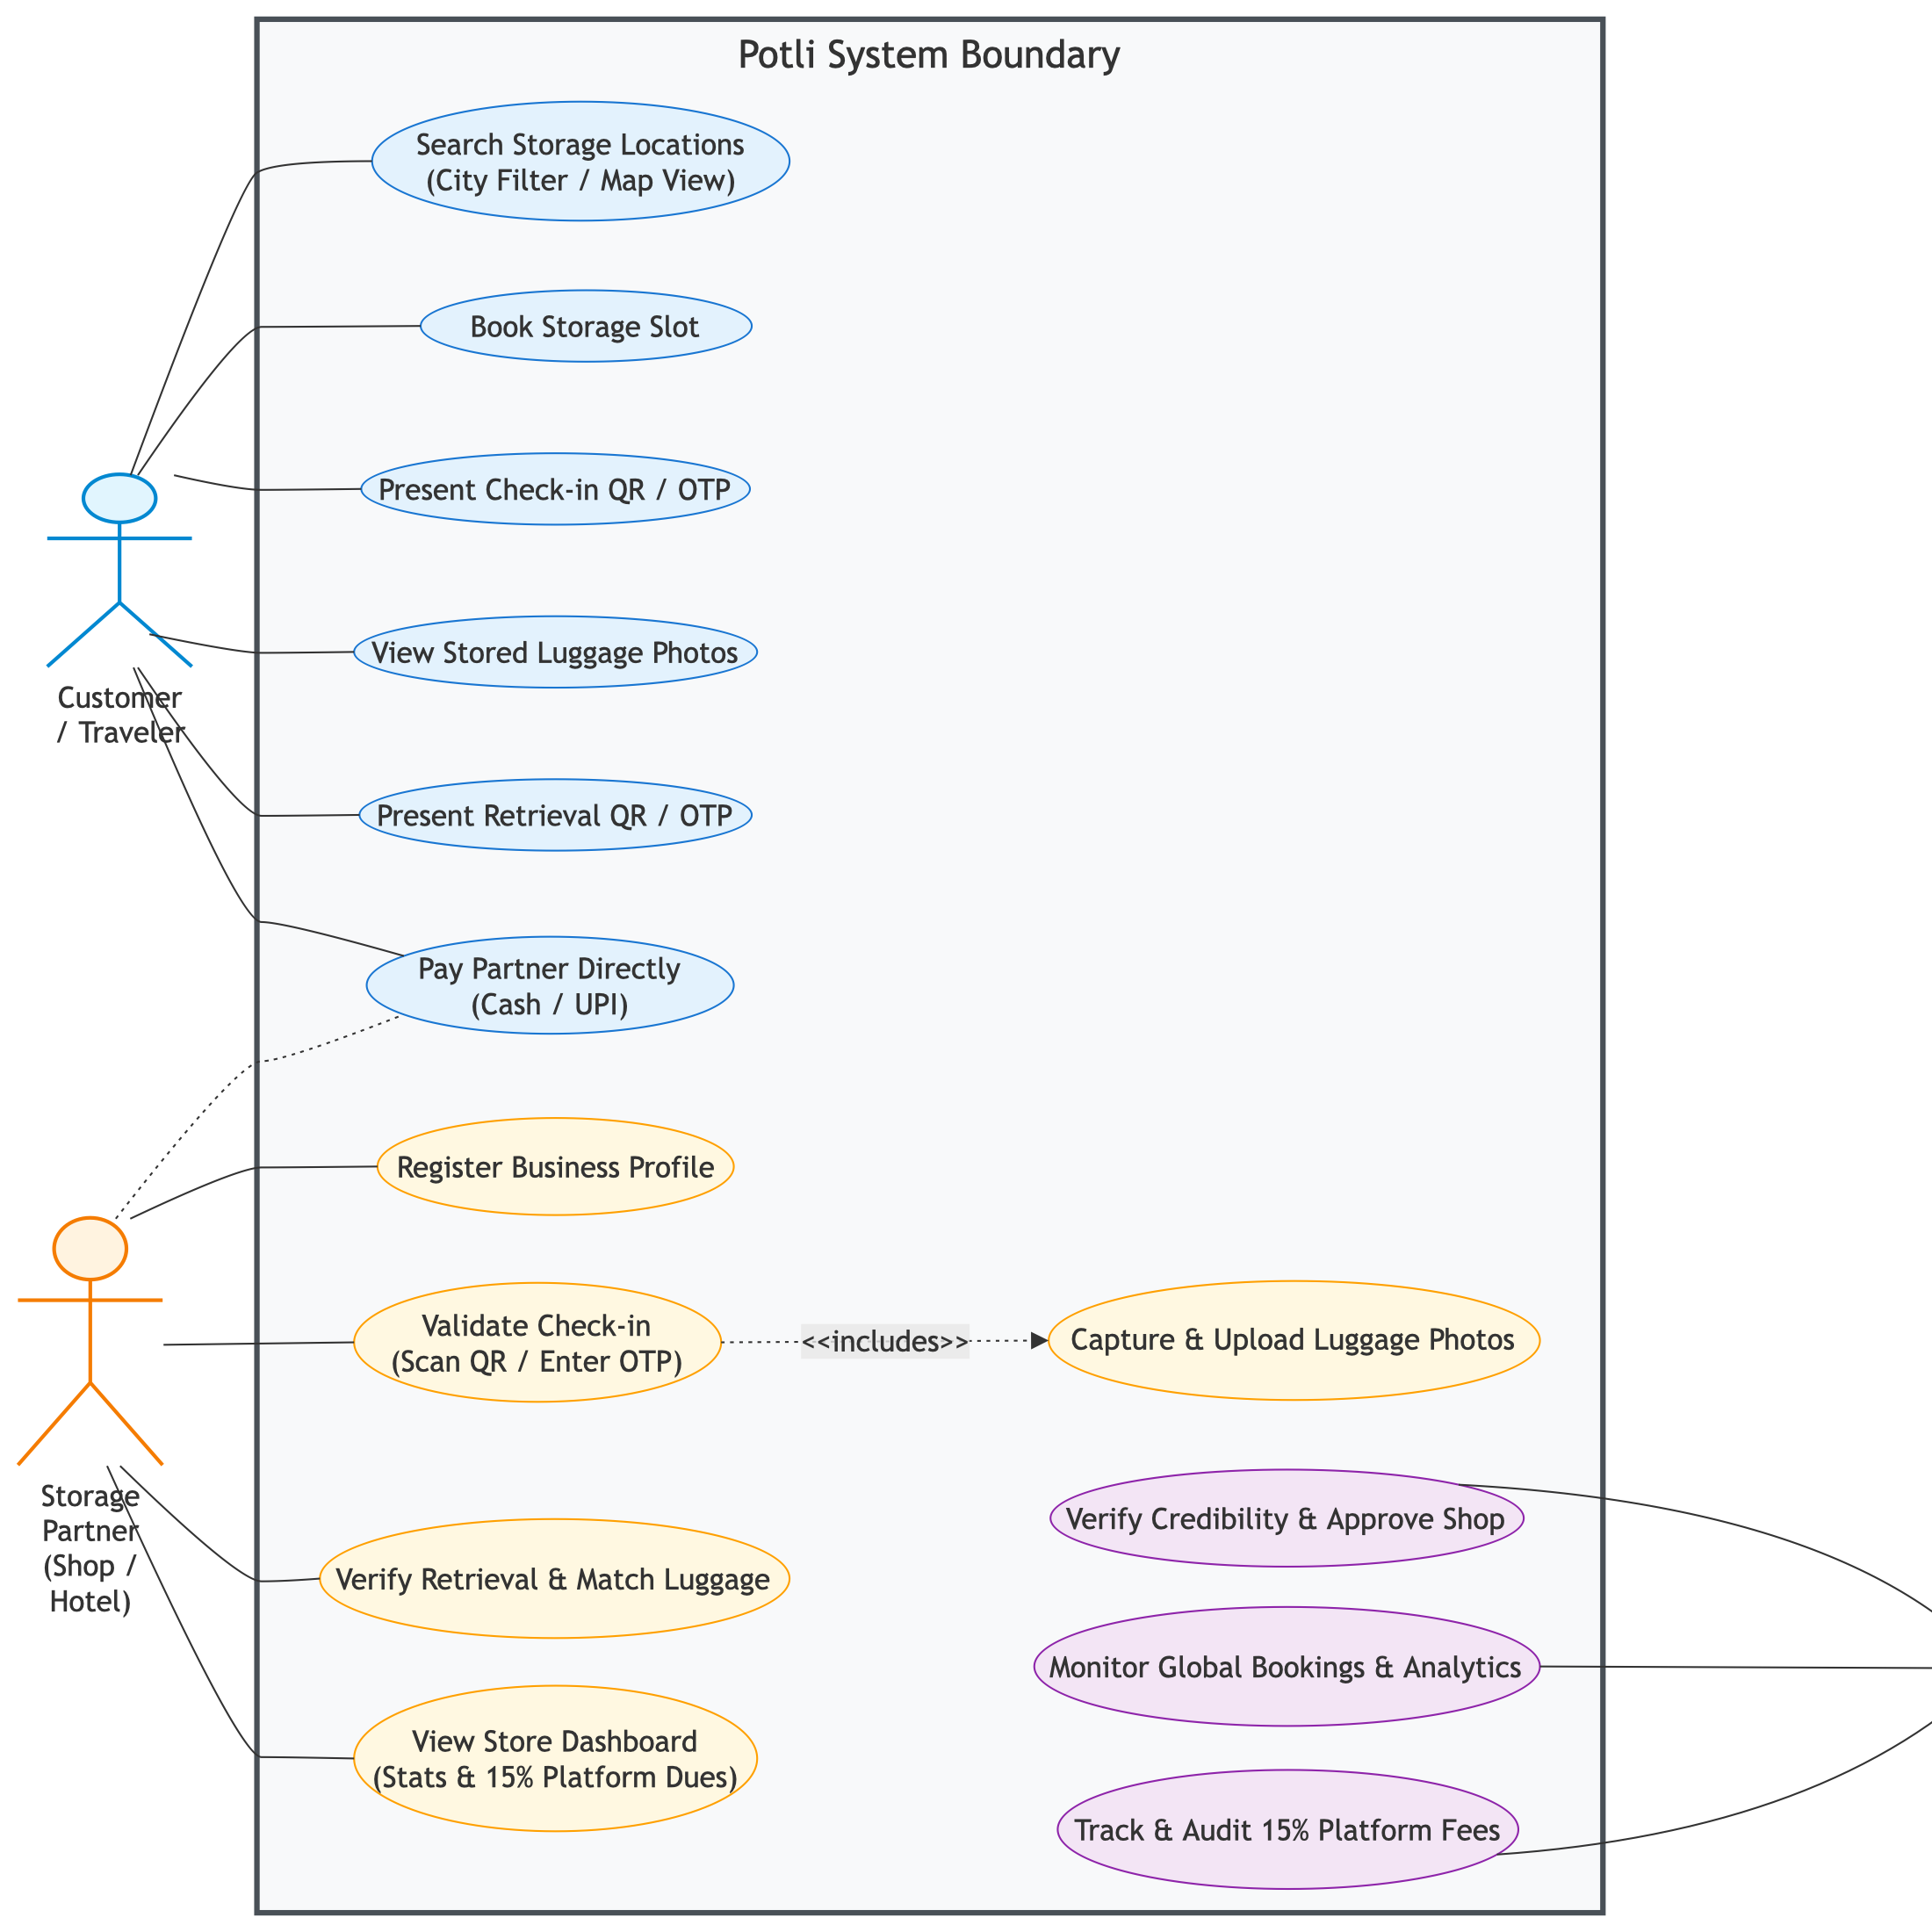
\includegraphics[width=0.88\textwidth,height=0.76\textheight,keepaspectratio]{use-case-diagram.png}
\caption{POTLI use-case diagram}
\label{fig:usecase}
\end{figure}

\section{Activity Model}
The activity diagram in Figure~\ref{fig:activity} follows the complete workflow across traveler, platform, storage partner, and administrator swimlanes. It includes partner approval, discovery, reservation, verification, storage, retrieval, and completion. The model is broader than the current prototype and acts as the implementation roadmap.

\begin{figure}[H]
\centering
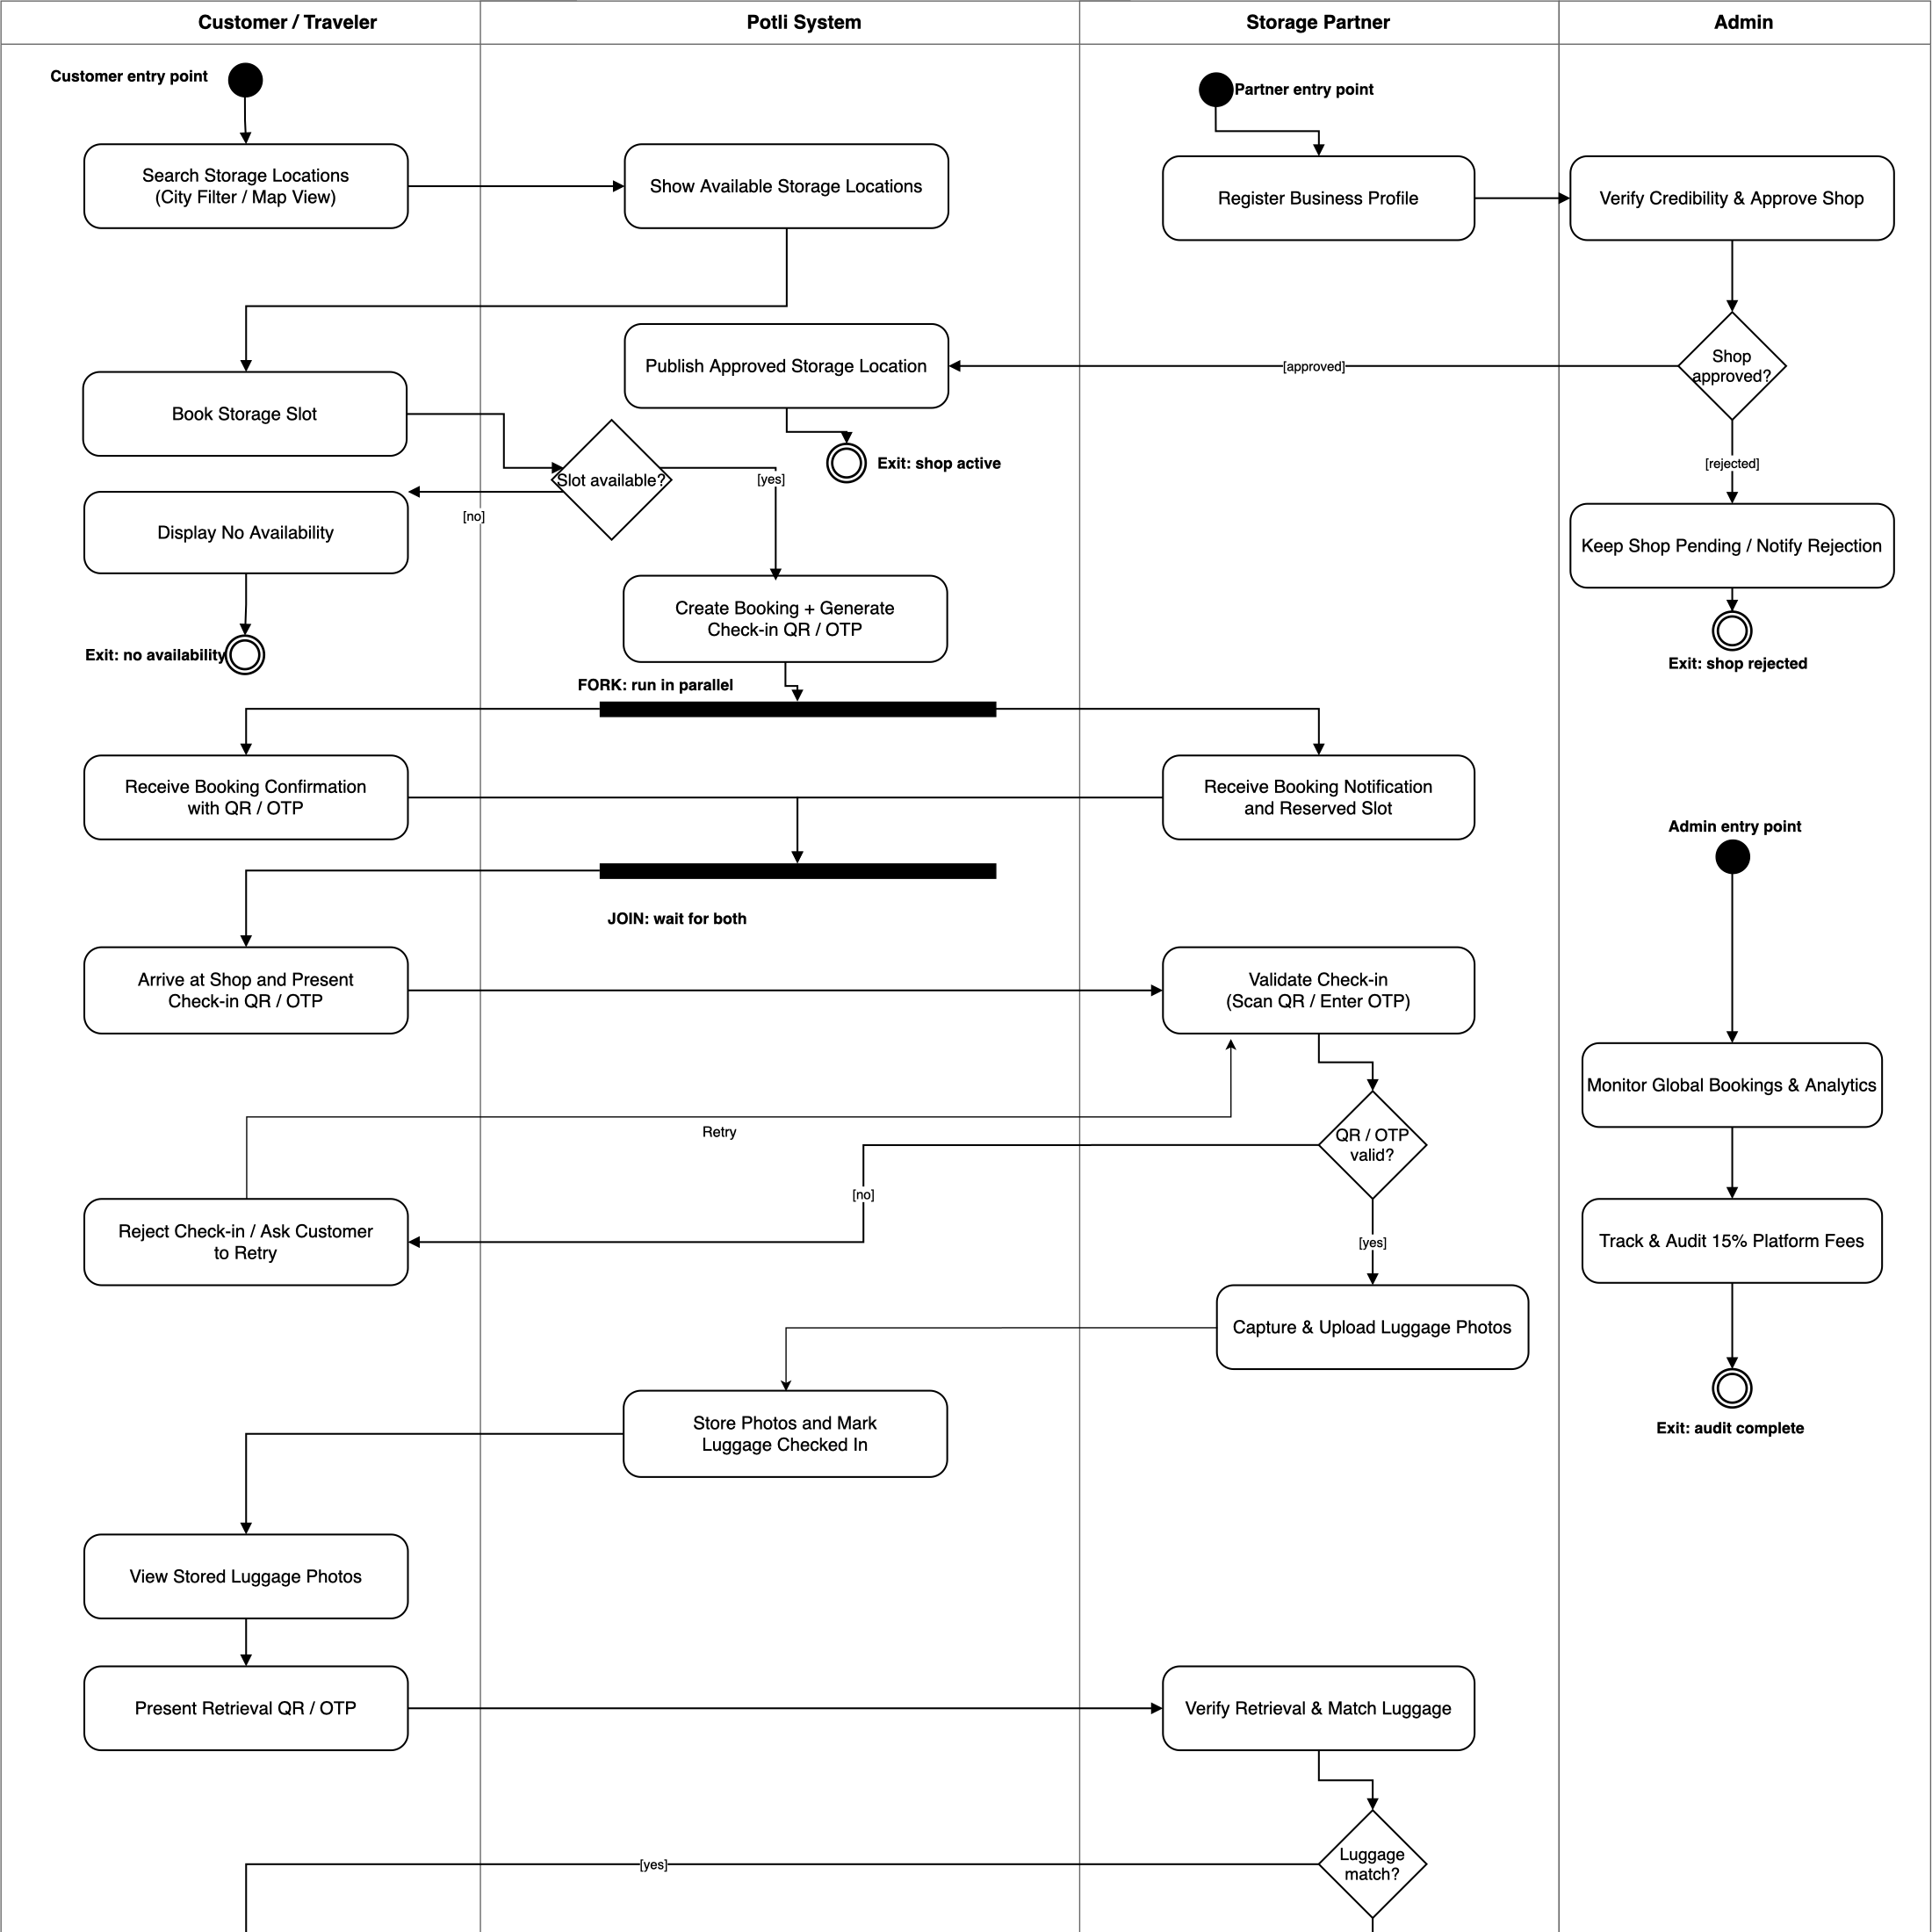
\includegraphics[width=0.88\textwidth,height=0.78\textheight,keepaspectratio]{activity-diagram.png}
\caption{End-to-end POTLI activity diagram}
\label{fig:activity}
\end{figure}

\chapter{Methodology and Design}

\section{Development Approach}
The project follows incremental delivery. The foundation increment establishes the interface, account model, authentication API, and database connectivity. Subsequent increments add listings and search, then booking and handoff state transitions, followed by partner/admin operations, payments, testing, and deployment. This sequence provides early demonstrable value while preserving traceability from requirements to implementation.

The Gantt chart in Figure~\ref{fig:gantt} organizes the work from requirements through launch demonstration. It should be read as the approved development plan rather than a claim that all activities are complete.

\begin{landscape}
\begin{figure}[H]
\centering
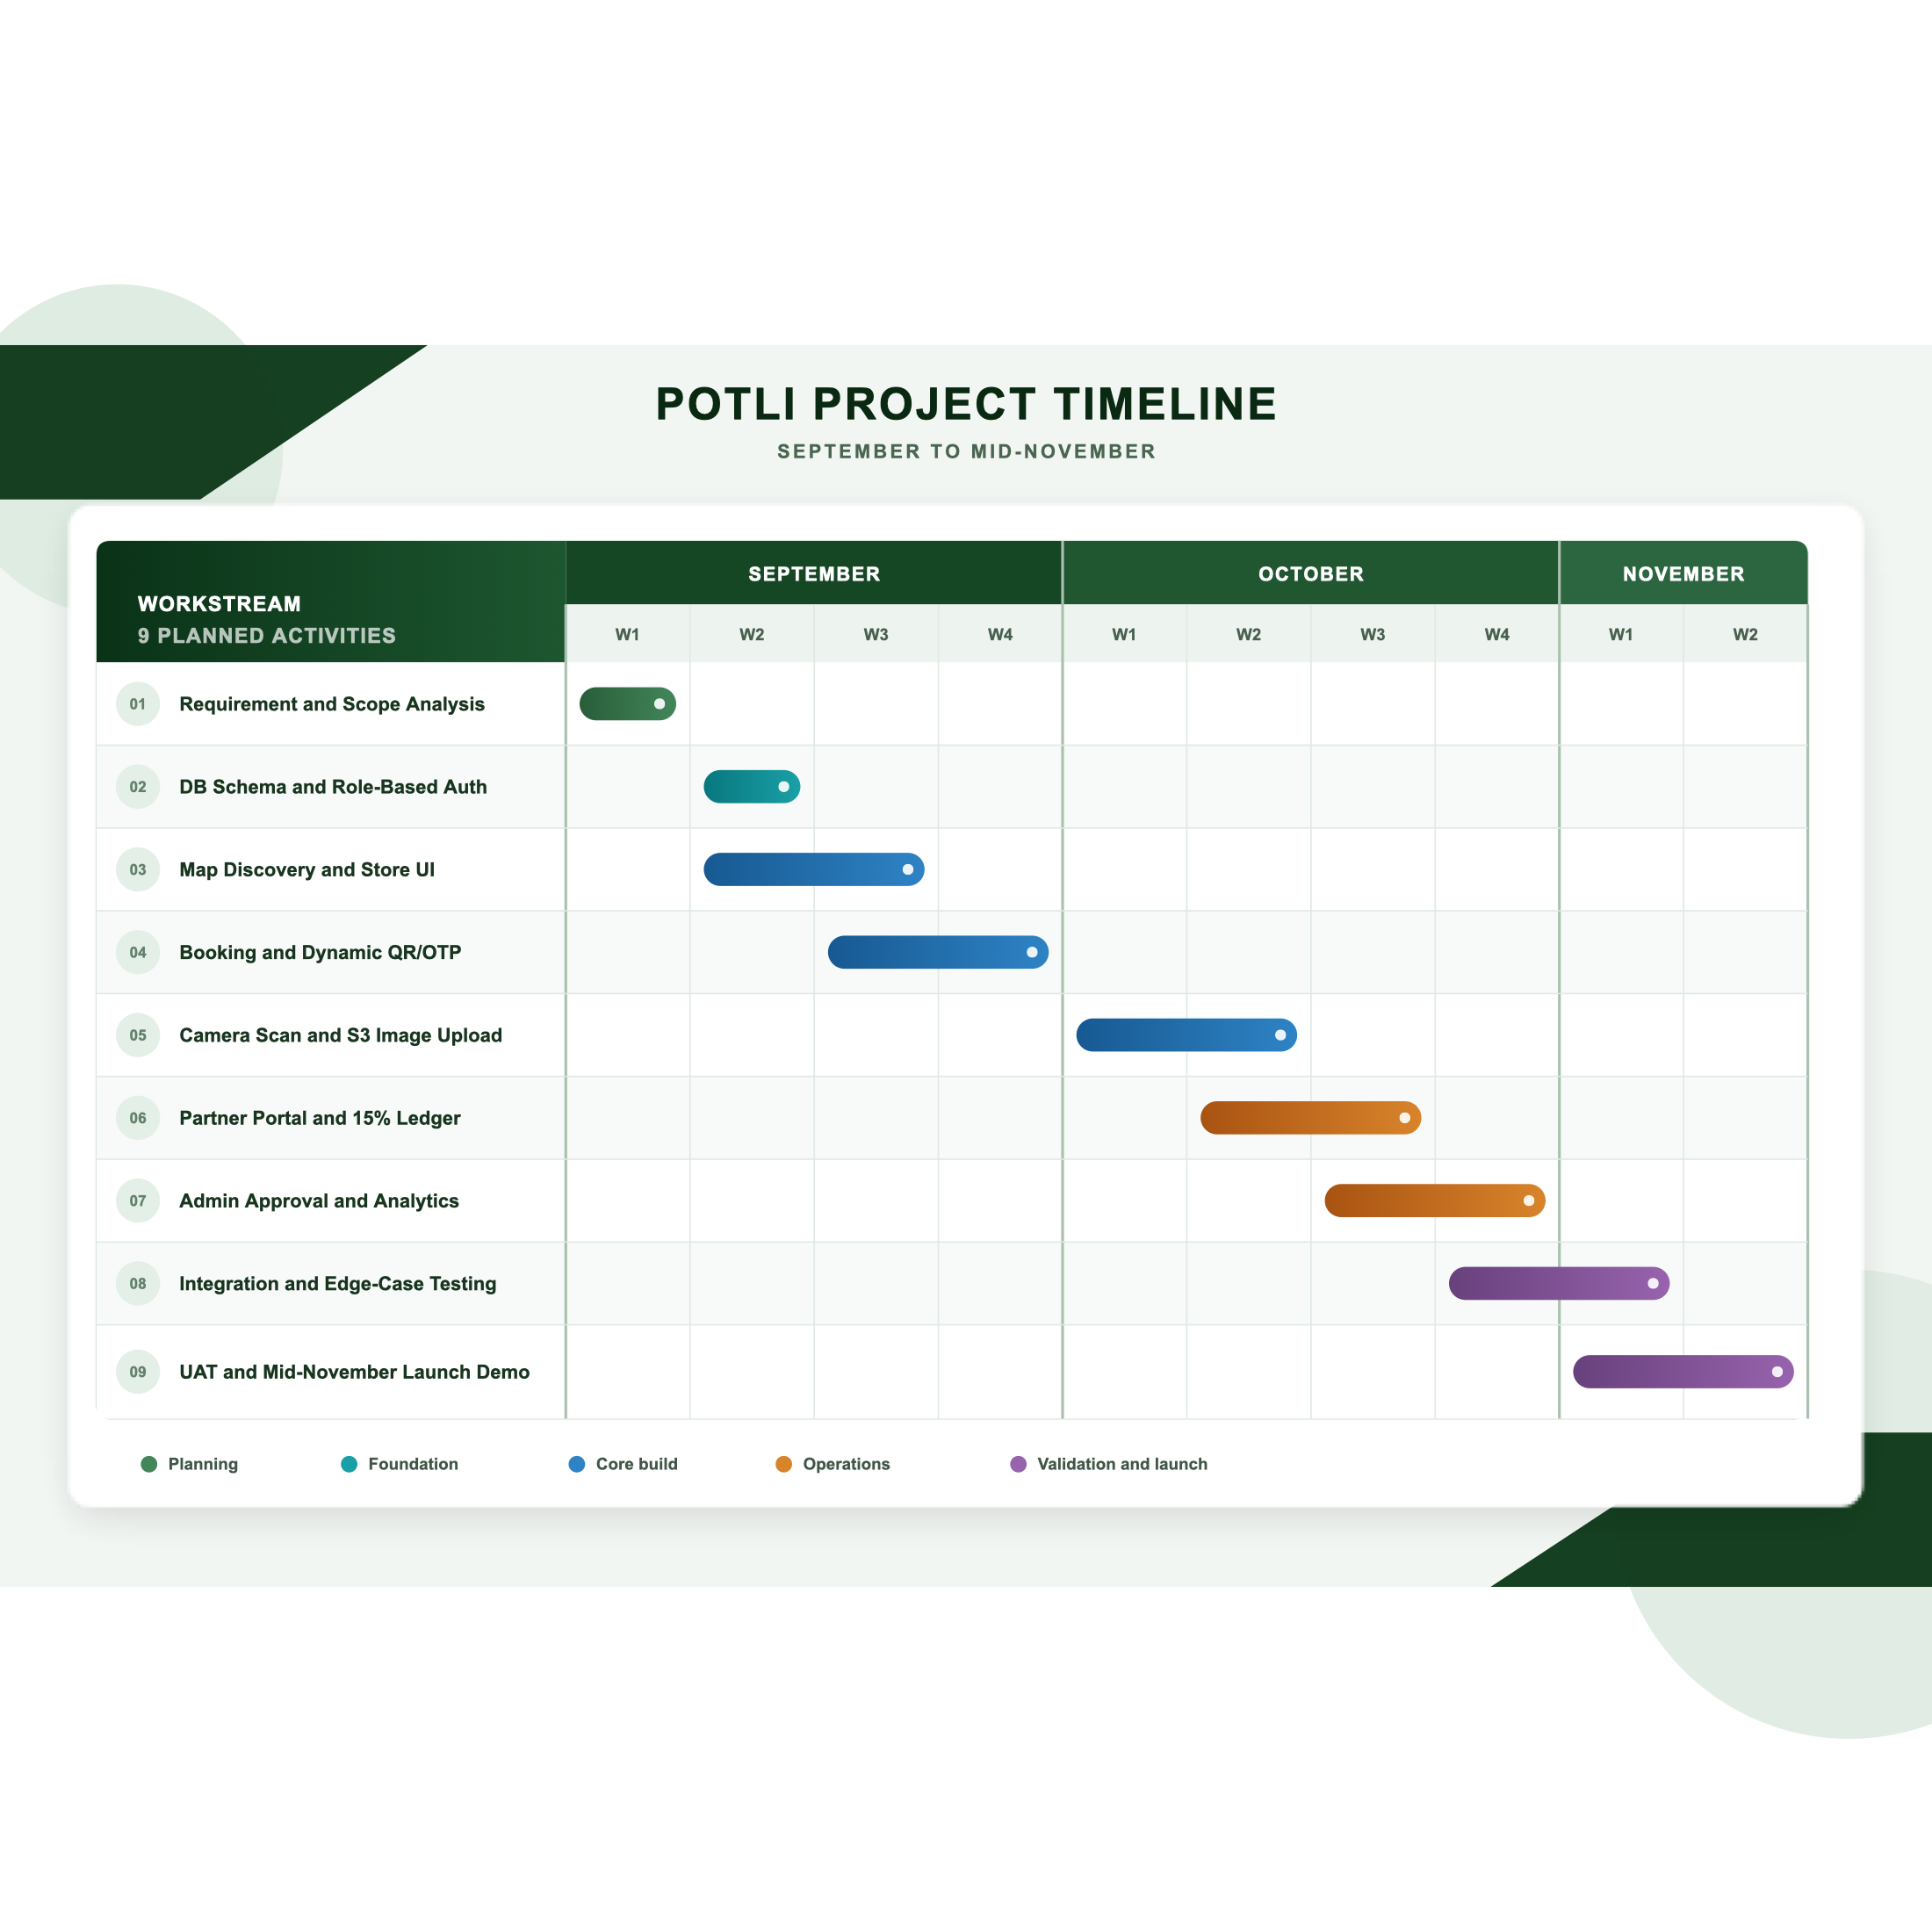
\includegraphics[width=0.94\linewidth,height=0.76\textheight,keepaspectratio]{gantt-chart.png}
\caption{Project development timeline}
\label{fig:gantt}
\end{figure}
\end{landscape}

\section{High-Level Architecture}
POTLI uses a three-tier web architecture:
\begin{enumerate}[leftmargin=*]
  \item \textbf{Presentation layer:} a responsive TypeScript application bundled with Vite~\cite{vite}. It renders route-specific pages and uses the Supabase JavaScript client to persist and refresh browser sessions.
  \item \textbf{Application layer:} a TypeScript Express~\cite{express} API. Implemented endpoints are grouped below \texttt{/api/v1}; deprecated unversioned aliases emit deprecation and sunset headers.
  \item \textbf{Data layer:} Supabase PostgreSQL~\cite{postgresql}, accessed through a shared Drizzle ORM workspace over the \texttt{pg} driver. Supabase Auth owns credentials, while public profile tables hold application roles and partner details.
\end{enumerate}

The browser signs in through Supabase Auth and receives a managed access/refresh-token session. It sends the access token to the API using the Bearer scheme; the API verifies it through Supabase, then loads the server-controlled role from the public profile. The API also exposes server-side login for non-browser clients. Search, booking, media storage, and payment integrations will extend this baseline.

\section{Data Flow Diagrams}
\subsection{Level 0: Context}
The Level 0 DFD (Figure~\ref{fig:dfd0}) treats POTLI as a single process. Registration, search, booking, business updates, administration, and payment data cross the system boundary through four external entities.

\begin{figure}[H]
\centering
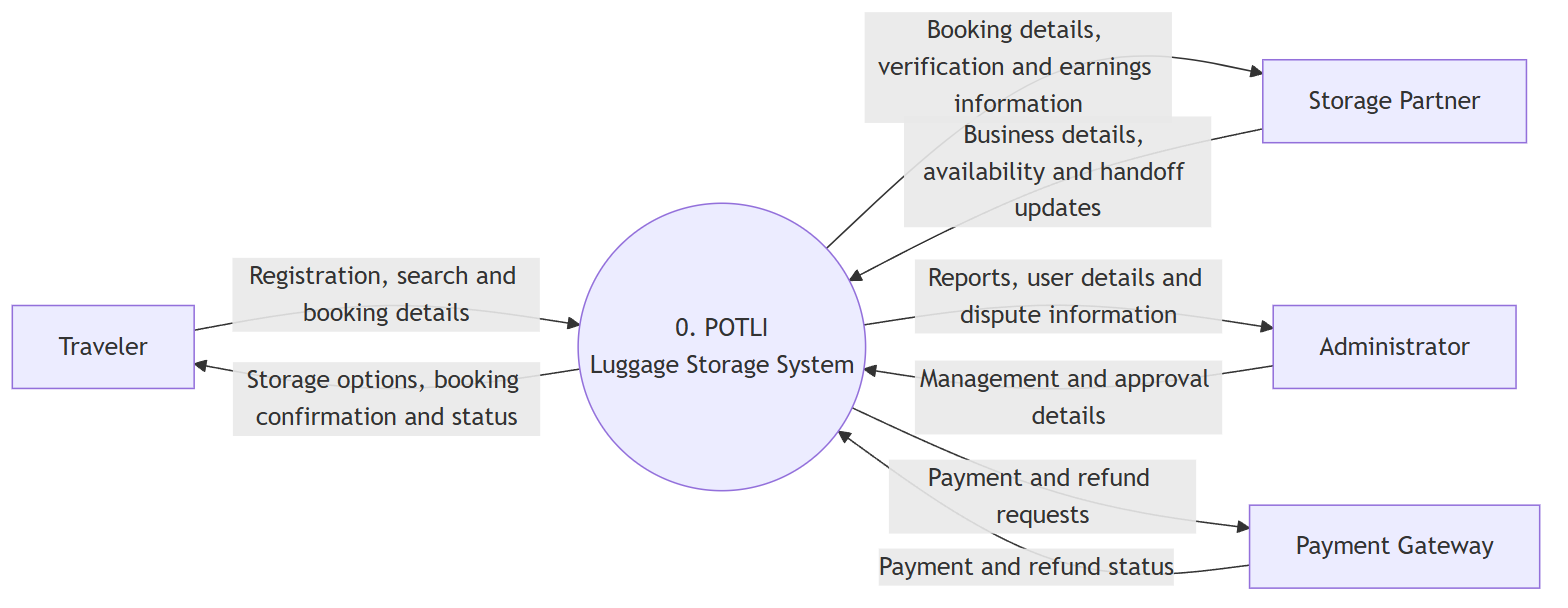
\includegraphics[width=\textwidth]{dfd-level-0.png}
\caption{Level 0 context data flow diagram}
\label{fig:dfd0}
\end{figure}

\subsection{Level 1: System Decomposition}
Figure~\ref{fig:dfd1} decomposes the platform into account management (1.0), storage listing management (2.0), bookings and handoffs (3.0), payment processing (4.0), and platform administration (5.0). Four conceptual stores hold user/partner data, listings, bookings, and payments.

\begin{landscape}
\begin{figure}[H]
\centering
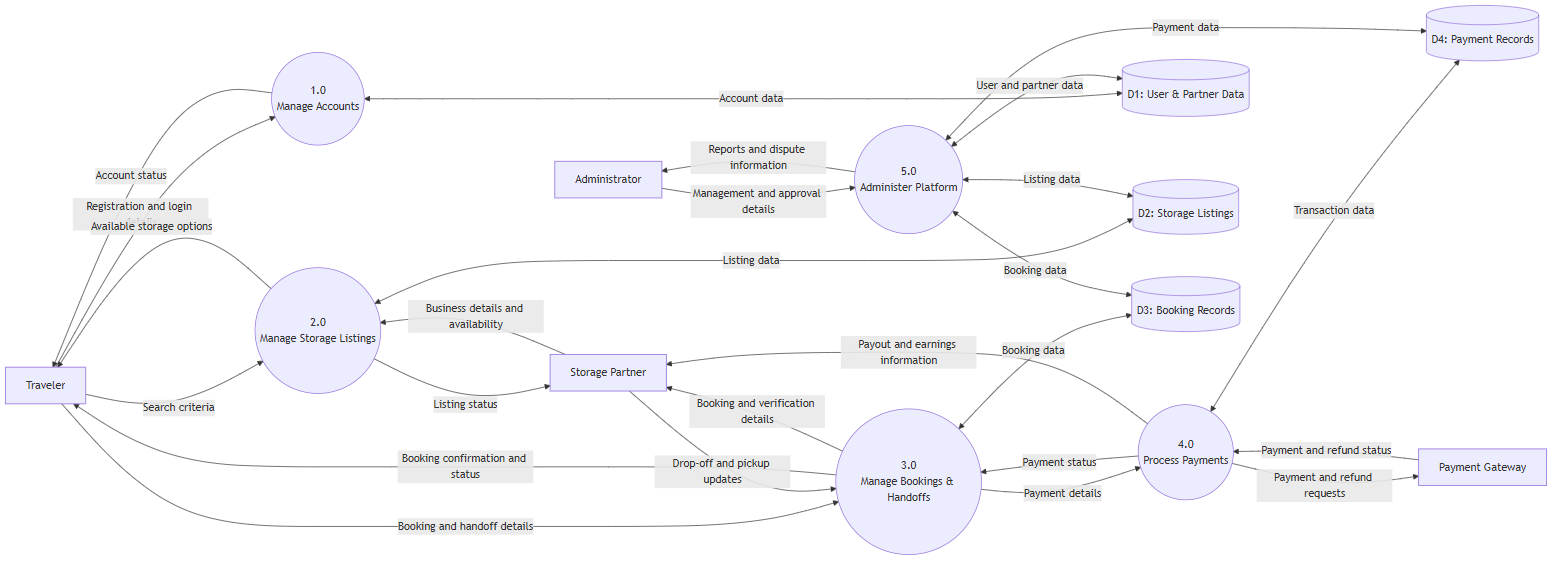
\includegraphics[width=0.97\linewidth]{dfd-level-1.png}
\caption{Level 1 system data flow diagram}
\label{fig:dfd1}
\end{figure}
\end{landscape}

\subsection{Level 2: Booking and Handoff}
The detailed DFD in Figure~\ref{fig:dfd2} expands process 3.0. A request is validated against listing data, a booking is created after payment status is received, the drop-off is verified and recorded, and pickup completes the booking while restoring capacity.

\begin{landscape}
\begin{figure}[H]
\centering
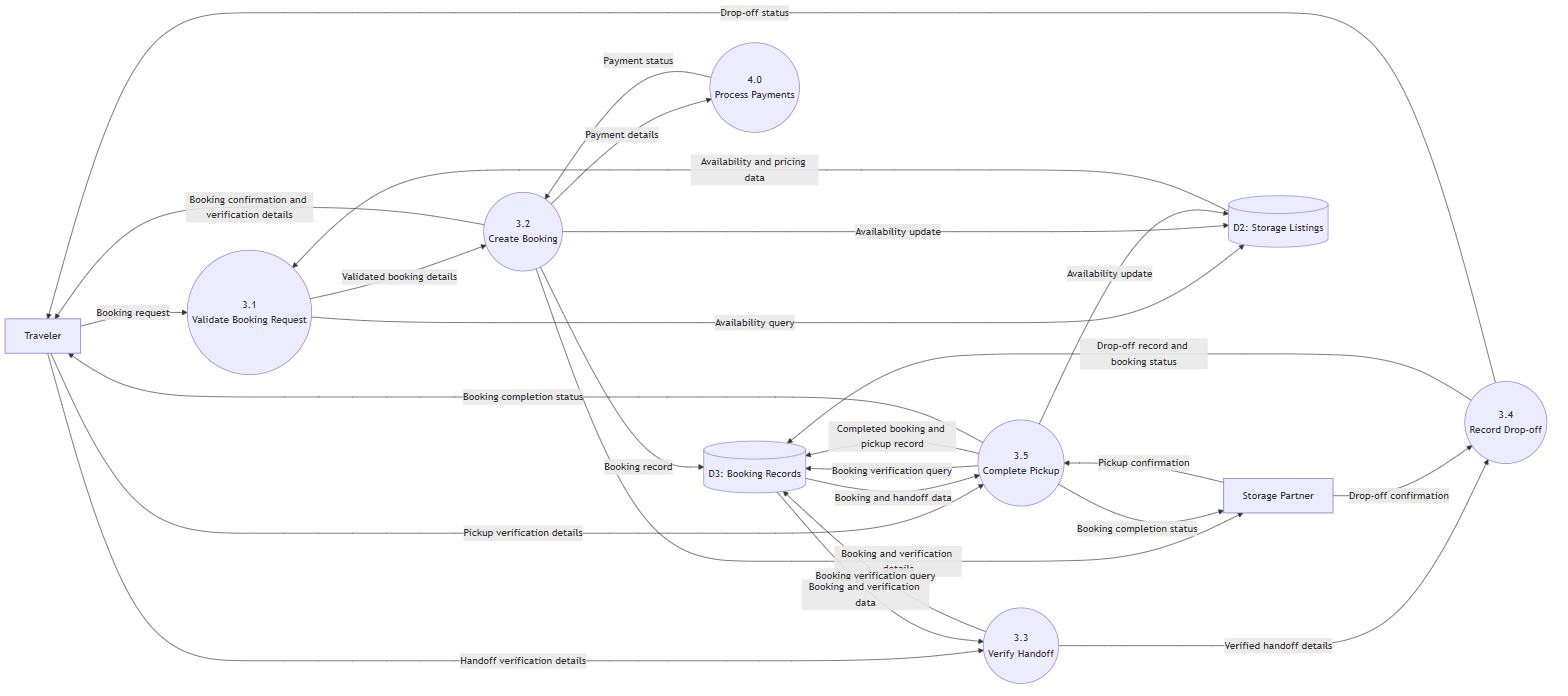
\includegraphics[width=0.97\linewidth]{dfd-level-2.png}
\caption{Level 2 booking and luggage-handoff data flow diagram}
\label{fig:dfd2}
\end{figure}
\end{landscape}

\section{Domain Model}
The class model in Figure~\ref{fig:class} connects the common \texttt{User} identity to traveler, partner, and administrator roles. It separates a partner's business profile from storage listings and composes booking records with handoff and payment information. Ratings remain optional because they occur after successful pickup.

\begin{figure}[H]
\centering
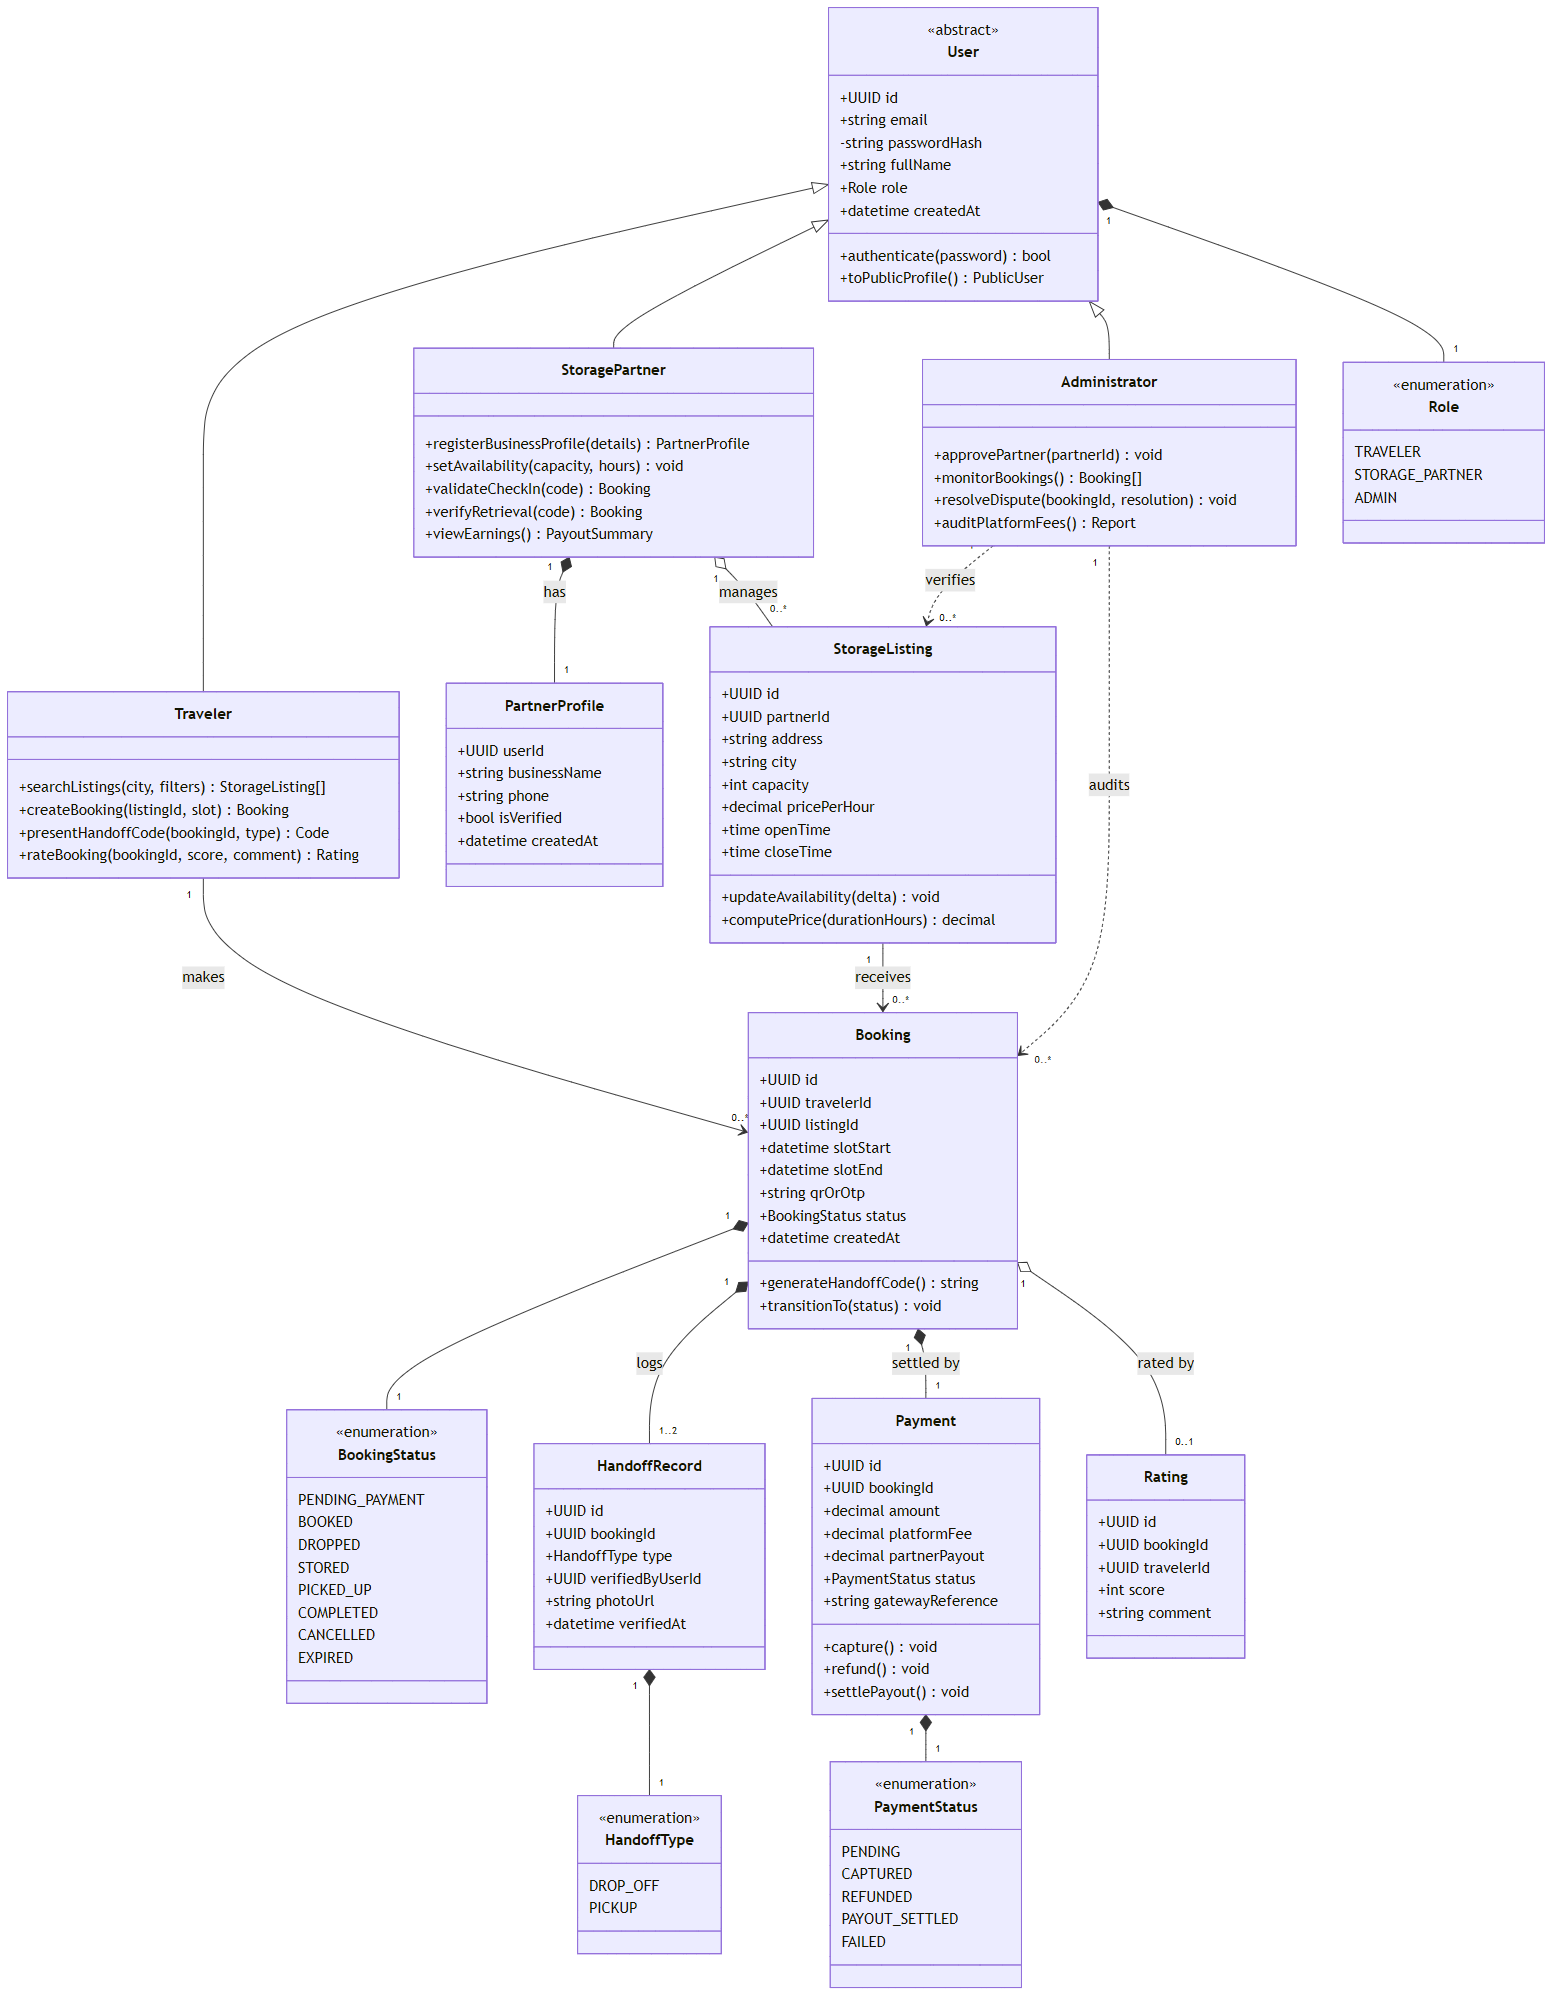
\includegraphics[width=0.82\textwidth,height=0.8\textheight,keepaspectratio]{class-diagram.png}
\caption{Planned POTLI domain class diagram}
\label{fig:class}
\end{figure}

\section{Behavioral Models}
\subsection{Sequence Diagram}
Figure~\ref{fig:sequence} shows the designed end-to-end interaction among traveler, web app, backend, database, payment gateway, and partner. The implemented login exchange appears within a larger planned sequence for discovery, booking, handoff, settlement, and rating.

\begin{figure}[H]
\centering
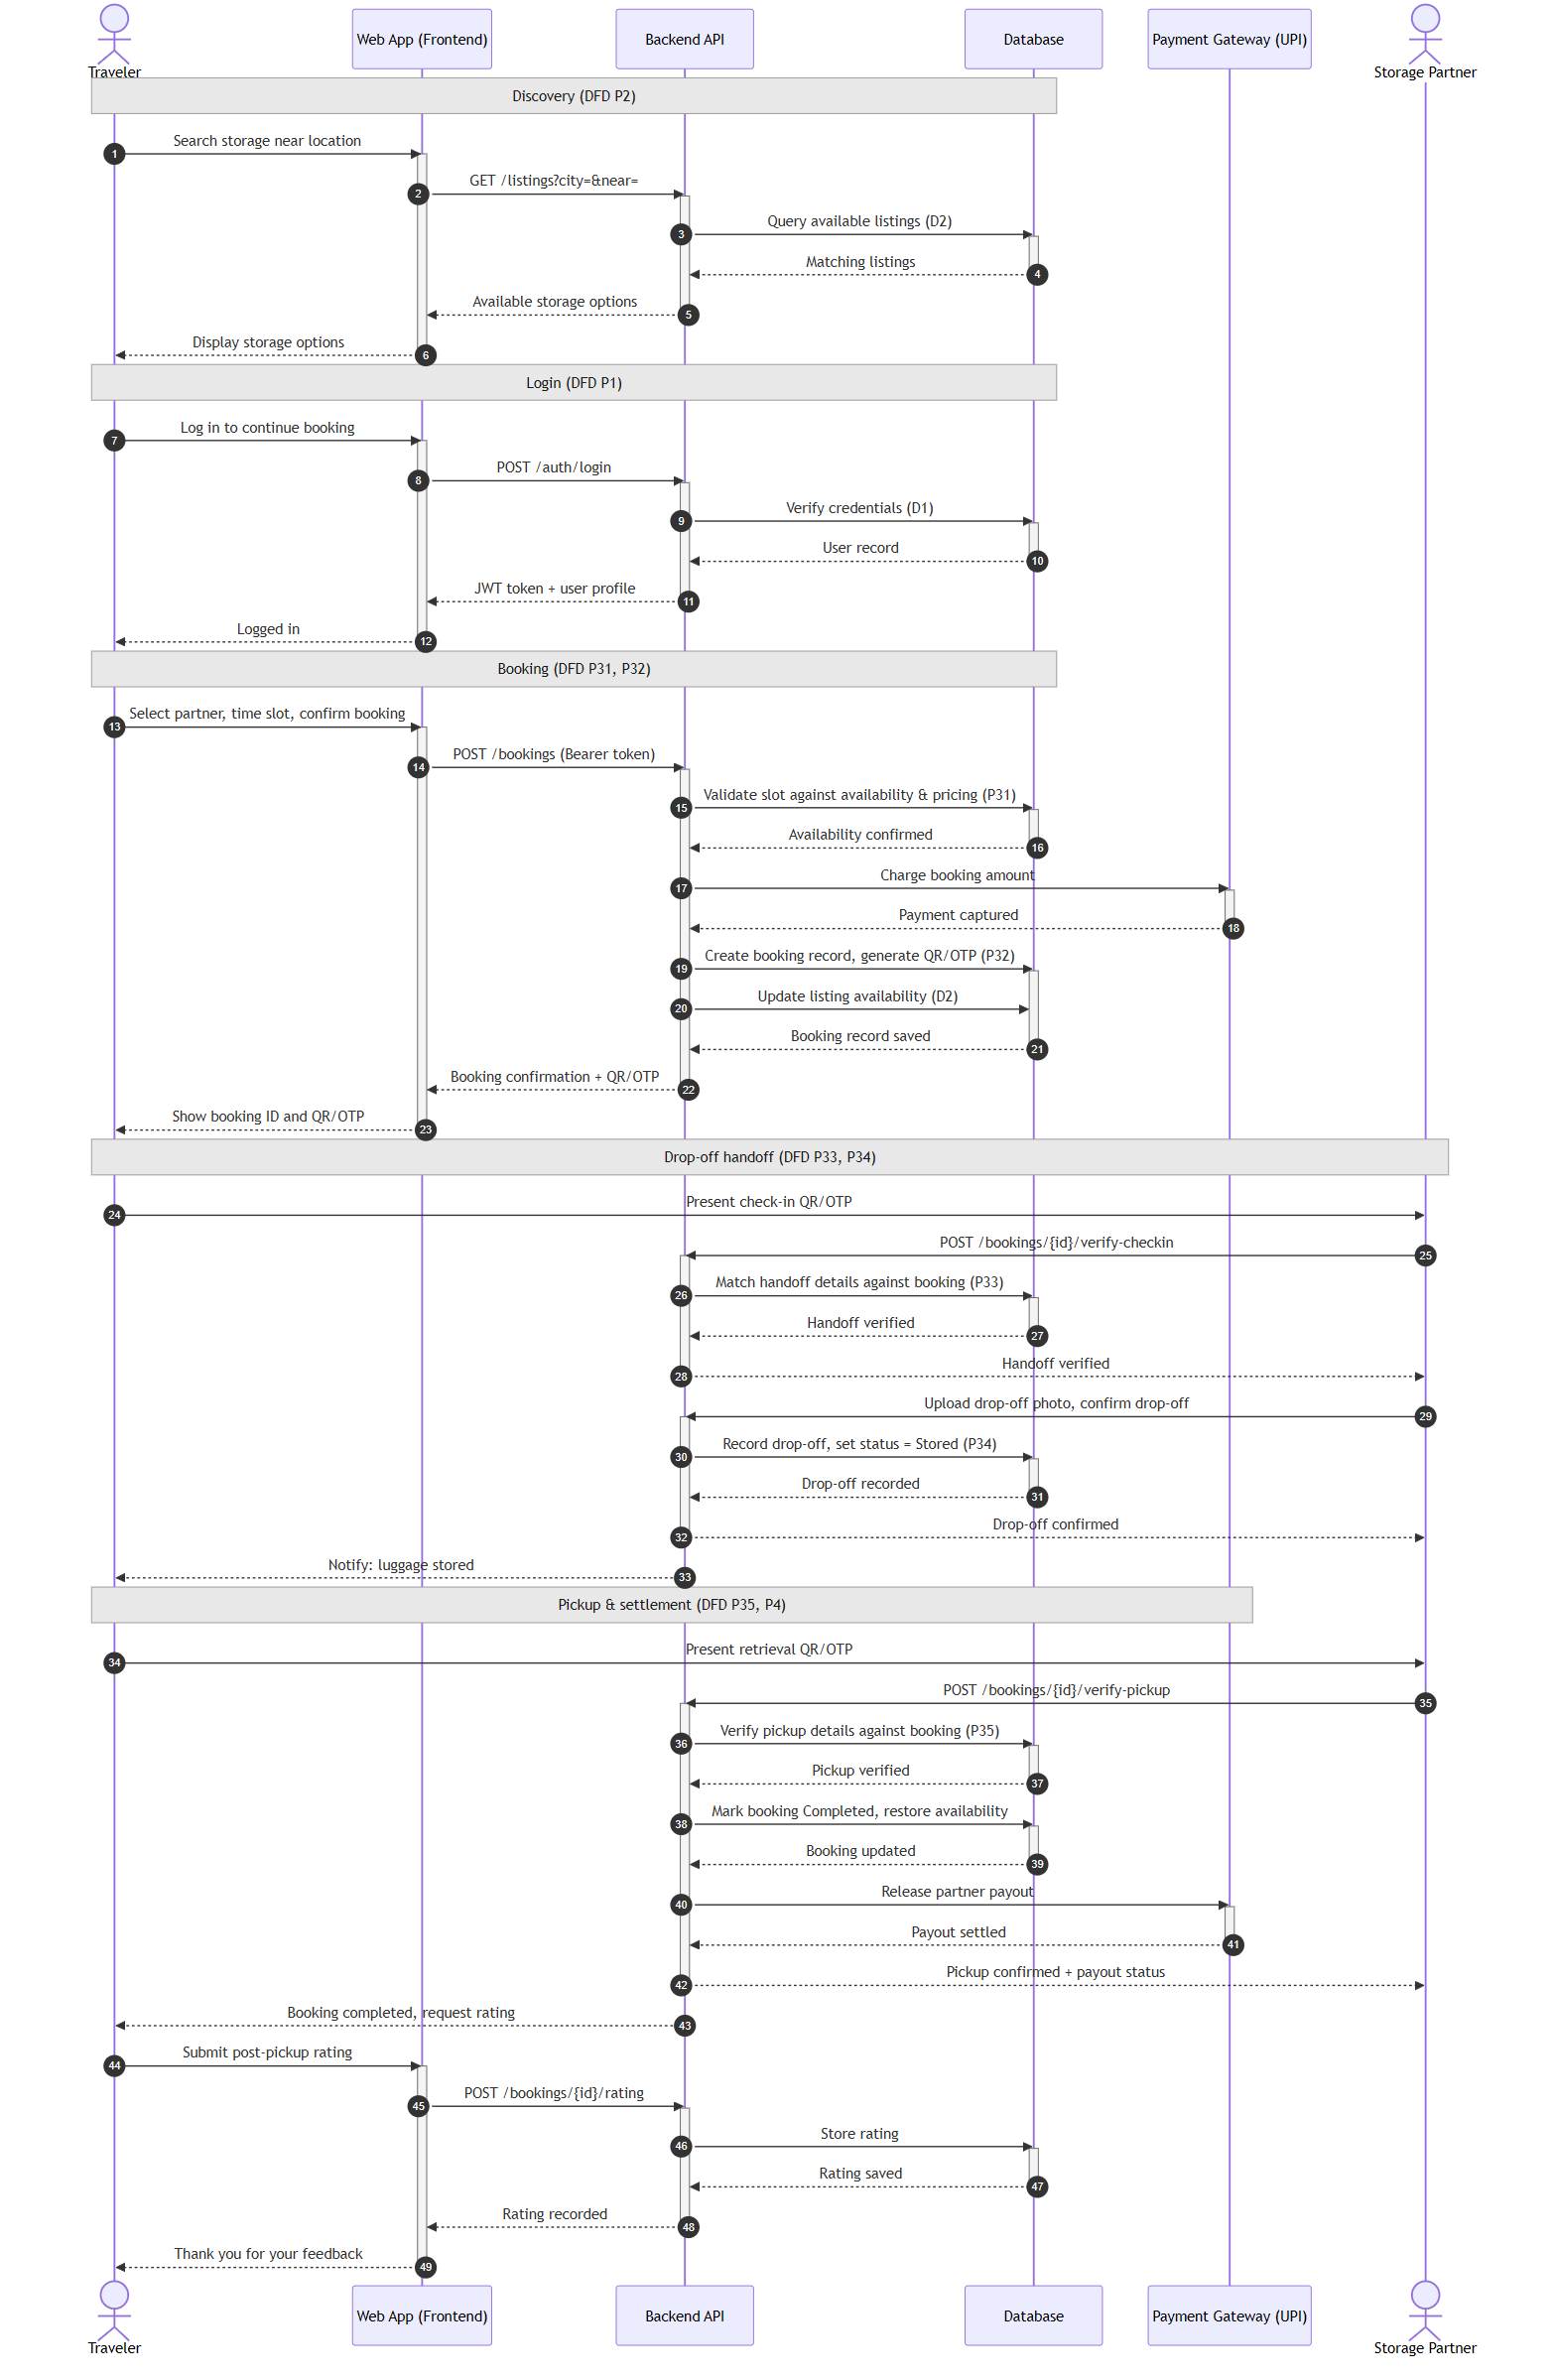
\includegraphics[width=0.78\textwidth,height=0.82\textheight,keepaspectratio]{sequence-diagram.png}
\caption{Booking and handoff sequence diagram}
\label{fig:sequence}
\end{figure}

\subsection{Collaboration Diagram}
The collaboration diagram (Figure~\ref{fig:collaboration}) presents the booking phase as numbered object-to-object messages rather than a time axis. It emphasizes the links among the web app, booking service, listing store, payment gateway, booking store, and partner.

\begin{landscape}
\begin{figure}[H]
\centering
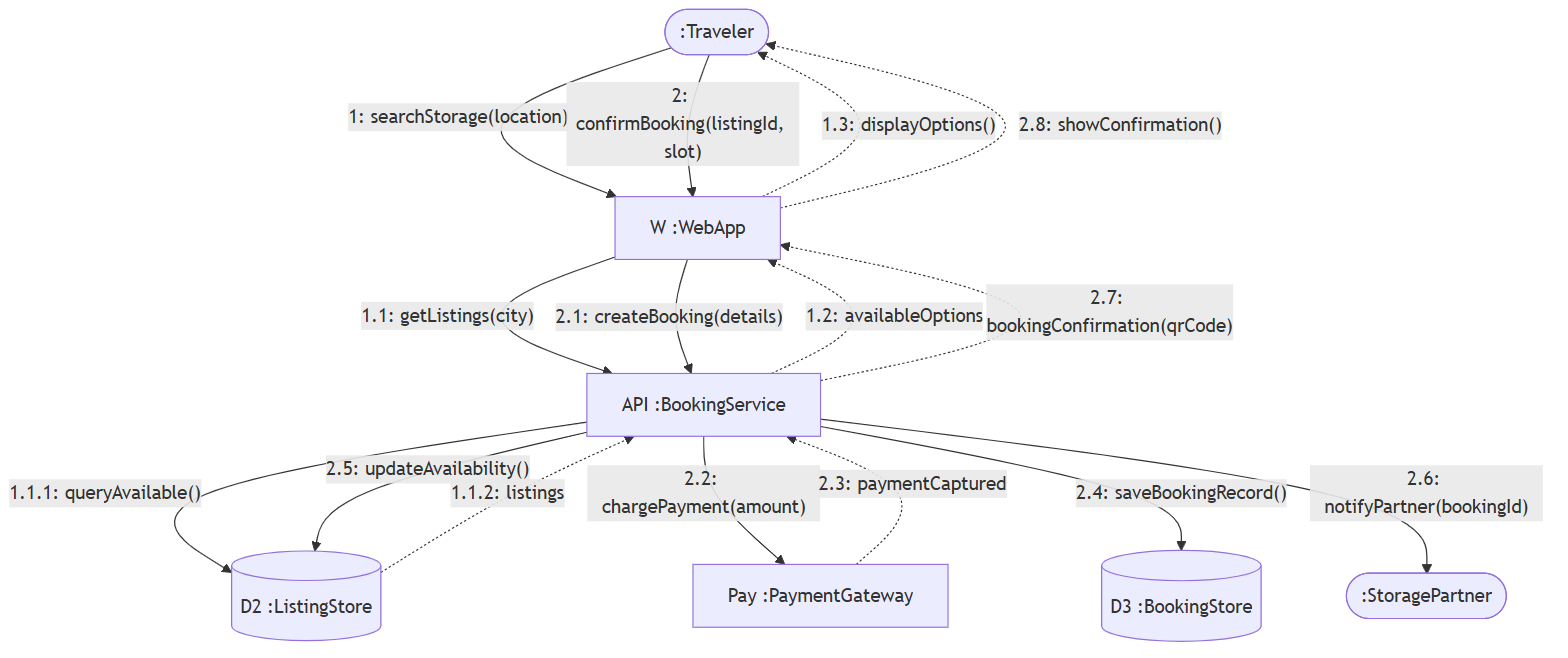
\includegraphics[width=0.95\linewidth]{collaboration-diagram.png}
\caption{Create-booking collaboration diagram}
\label{fig:collaboration}
\end{figure}
\end{landscape}

\subsection{State Diagram}
The booking state machine in Figure~\ref{fig:state} makes valid transitions explicit. A validated request enters \texttt{PendingPayment}; successful capture creates \texttt{Booked}; verified handoffs lead through \texttt{Dropped}, \texttt{Stored}, and \texttt{PickedUp}; payout settlement produces \texttt{Completed}. Failed payment, cancellation, or a missed slot enters a terminal exception state.

\begin{figure}[H]
\centering
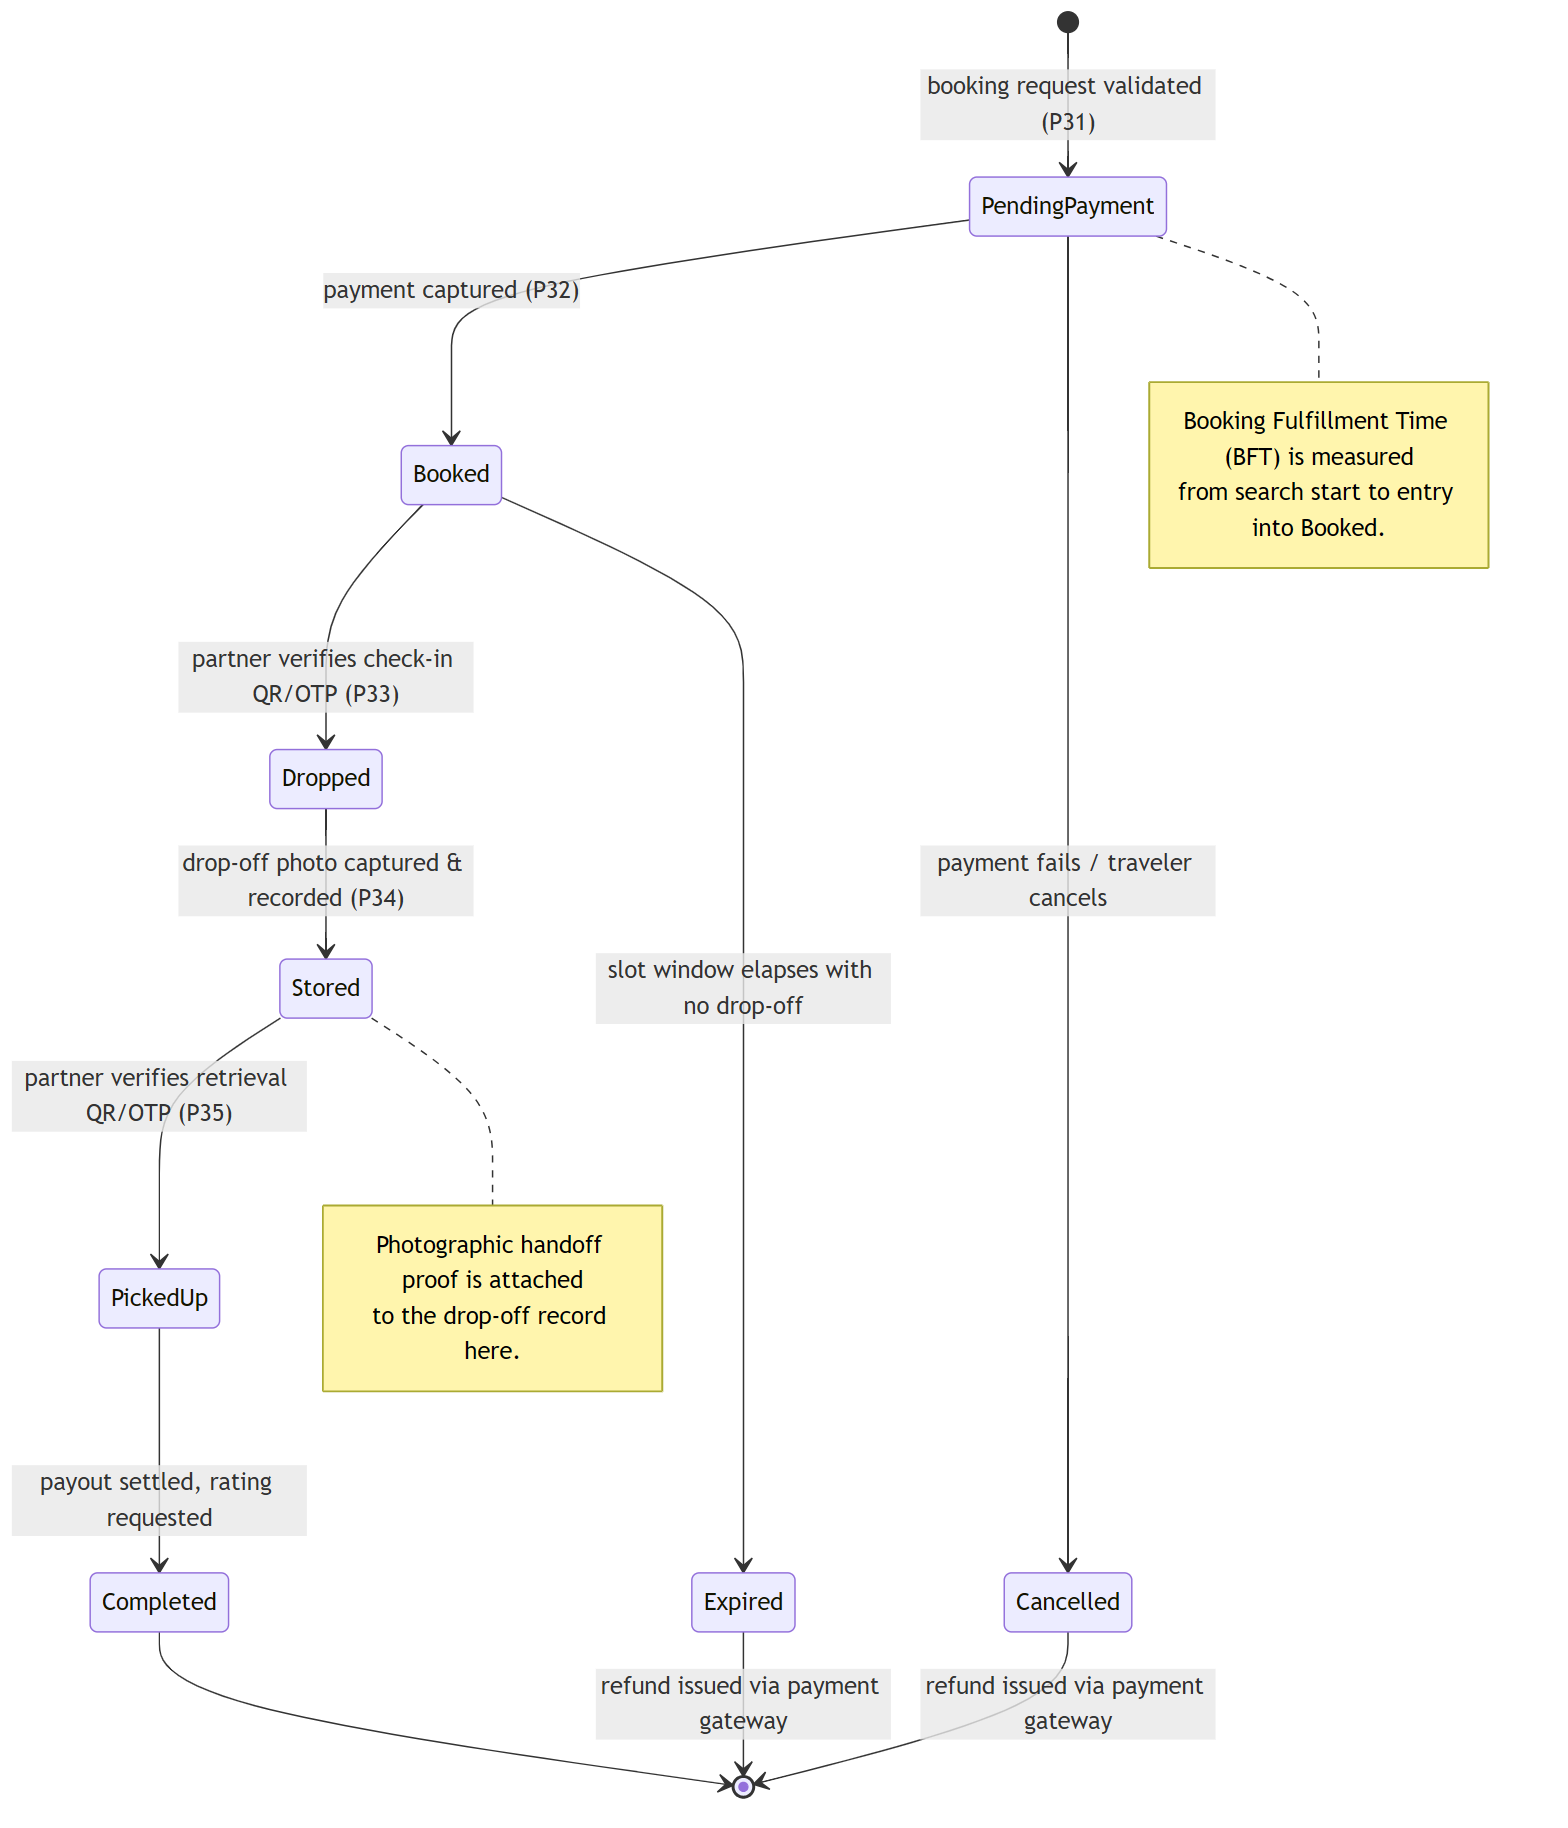
\includegraphics[width=0.76\textwidth,height=0.8\textheight,keepaspectratio]{state-diagram.png}
\caption{Booking lifecycle state diagram}
\label{fig:state}
\end{figure}

\chapter{Implementation Details}

\section{Frontend Prototype}
The frontend is a Vite project written in TypeScript and styled with a custom responsive stylesheet. A single rendering entry point maps URL hashes to the landing page, traveler login, admin login, partner account page, or role dashboard. Reusable inline SVG icons, semantic forms, labels, status messages, and navigation links reduce external UI dependencies.

The landing experience communicates the service model, trust controls, partner proposition, and project team. Authentication forms use \texttt{supabase-js}, which persists and refreshes the session, and then call the versioned backend to load the public role profile. The role dashboard changes its copy for traveler, storage partner, or administrator, and each sign-in route rejects credentials for an incompatible role. Search submission and new partner registration are currently interface demonstrations; they do not yet create persistent domain records.

\section{Backend Authentication API}
The backend uses TypeScript on Node.js and Express with CORS and JSON middleware. Its main implemented responsibilities are:
\begin{itemize}[leftmargin=*]
  \item checking database availability through \texttt{GET /api/v1/health};
  \item validating email/password credentials through \texttt{POST /api/v1/auth/login};
  \item delegating credential checks and token issuance to Supabase Auth;
  \item verifying a bearer token, loading its public profile, and returning the user through \texttt{GET /api/v1/auth/me}; and
  \item retaining temporary unversioned aliases with explicit deprecation metadata.
\end{itemize}

Database access is centralized in the shared Drizzle workspace. Credentials and token signing remain owned by Supabase Auth; the backend uses the publishable key to verify tokens and does not require a service-role secret. Asynchronous route failures reach centralized error handling rather than terminating the process.

\section{Database Schema}
Supabase Auth owns \texttt{auth.users} and its credential records. A Drizzle-defined public \texttt{profiles} table references each auth UUID and stores email, full name, a constrained \texttt{traveler}/\texttt{storage\_partner}/\texttt{admin} role, and timestamps. The \texttt{partner\_profiles} table extends partner accounts with business name and phone number using a cascading foreign key. A signup trigger creates traveler profiles, while row-level security allows users to read their own profile and administrators to read all profiles.

Later migrations will introduce the designed D2--D4 stores: listings and capacity, bookings and handoff records, and payment/settlement records. Transactional constraints will be required so simultaneous requests cannot reserve the same final unit of capacity.

\section{Security and Privacy Considerations}
The prototype delegates password hashing and signed sessions to Supabase Auth and protects profile access with row-level security, but a deployable service requires additional controls. These include rate limiting, generic authentication errors, refresh/revocation strategy, secure cookie evaluation in place of unrestricted local storage, authorization middleware for every protected role, strict request schemas, TLS, audit logs, and controlled access to handoff photographs. Personally identifiable information and location history should be minimized and retained only for defined operational periods.

\chapter{Testing and Evaluation}

\section{Testing Methodology}
The planned verification strategy combines:
\begin{itemize}[leftmargin=*]
  \item \textbf{Unit tests} for validation, status transitions, pricing, token handling, and utility functions;
  \item \textbf{API integration tests} against an isolated PostgreSQL database for login, authorization, booking races, handoff codes, and invalid transitions;
  \item \textbf{Frontend tests} for route rendering, form behavior, error handling, responsive layout, and accessibility;
  \item \textbf{End-to-end tests} for traveler booking through partner pickup and administrator review;
  \item \textbf{Performance tests} for nearby search and concurrent booking creation; and
  \item \textbf{Pilot user testing} with representative travelers and local businesses.
\end{itemize}

\section{Current Verification Status}
At the mid-semester stage, root workspace scripts support full TypeScript checking, a deterministic frontend production build, and an idempotent Supabase migration/seed workflow. The backend does not yet contain an automated test suite, and live API verification depends on a configured PostgreSQL connection. Accordingly, no fabricated accuracy, throughput, uptime, or pilot figures are reported here.

\begin{table}[H]
\centering
\begin{tabular}{p{0.32\textwidth}p{0.22\textwidth}p{0.36\textwidth}}
\toprule
\textbf{Check} & \textbf{Status} & \textbf{Interpretation} \\
\midrule
TypeScript compilation and Vite production build & Available & Detects type/build failures and produces deployable static assets \\
Database migration and seed scripts & Available & Creates development roles when a valid database URL is supplied \\
Automated backend unit/integration suite & Not yet implemented & Required before release readiness can be claimed \\
End-to-end booking workflow & Not yet testable & Booking and handoff modules remain planned \\
Pilot performance measurements & Not yet collected & Must follow implementation and field trial \\
\bottomrule
\end{tabular}
\caption{Mid-semester verification status}
\label{tab:verification}
\end{table}

\section{Evaluation Metrics}
\begin{table}[H]
\centering
\begin{tabular}{p{0.30\textwidth}p{0.20\textwidth}p{0.40\textwidth}}
\toprule
\textbf{Metric} & \textbf{Target} & \textbf{Measurement} \\
\midrule
Median Booking Fulfillment Time & $\leq 3$ minutes & Search-start timestamp to confirmed-booking timestamp \\
Handoff success rate & Establish after pilot & Completed drop-off and pickup without dispute / initiated handoffs \\
Partner utilization & Establish baseline & Booked capacity / listed capacity per partner-week \\
Payout turnaround & Define with gateway & Completion timestamp to credited-payout timestamp \\
Traveler satisfaction & 1--5 scale & Post-pickup rating and short qualitative feedback \\
Business-hour availability & $\geq 99\%$ pilot goal & Successful health/search probes during defined hours \\
\bottomrule
\end{tabular}
\caption{Proposed evaluation metrics}
\label{tab:metrics}
\end{table}

\section{Pilot Plan}
A small locality near a railway station or busy market can provide a controlled first deployment. The proposed pilot includes 8--12 partner businesses and 15--20 traveler participants. Before use, partners receive a brief handoff procedure and the team confirms business details. Application timestamps provide quantitative measures, while structured post-use questions capture convenience, trust, and onboarding difficulty. Any safety incident or disputed handoff takes priority over performance measurement.

\chapter{Conclusion}

\section{Summary of Work}
POTLI defines a practical web platform for connecting travelers who need short-term luggage storage with local businesses that can provide it. The project has progressed from proposal and requirements into a documented architecture, balanced DFDs, UML behavioral and structural models, a responsive frontend prototype, a versioned Express authentication API, and a PostgreSQL role schema.

The current implementation proves the foundation rather than the complete service. Its strongest completed elements are role-aware account access, API/database connectivity, a coherent user experience, and detailed traceable system design. Core transactional capabilities---search-backed listings, reservations, QR/OTP handoffs, payment settlement, ratings, and administrative operations---remain future increments.

\section{Key Findings}
\begin{itemize}[leftmargin=*]
  \item Trust must be represented as verifiable workflow data: identity review, explicit state transitions, handoff credentials, timestamps, and photographic evidence.
  \item Availability and booking creation form the central consistency boundary; they must be updated transactionally to prevent overbooking.
  \item A shared user table with constrained roles simplifies authentication, while separate partner profiles and domain tables preserve extensibility.
  \item The BFT target is useful only when timestamps and state definitions are implemented before pilot measurement.
\end{itemize}

\section{Future Work and Recommendations}
\begin{enumerate}[leftmargin=*]
  \item Implement listing management and indexed location search.
  \item Add transactional booking creation and dynamic QR/OTP credentials.
  \item Build protected partner handoff screens with secure photo upload.
  \item Introduce role-authorization middleware and comprehensive automated tests.
  \item Integrate a sandbox payment gateway before enabling real collections or payouts.
  \item Build administrator verification, audit, analytics, and dispute tools.
  \item Deploy a staging environment, run the proposed pilot, and replace target values with measured results.
\end{enumerate}

\section{Final Remarks}
The project is technically feasible with established web components, but its success depends as much on operational clarity and trust as on interface quality. The next milestone should prioritize one complete, tested path from available listing to verified pickup before broadening features. This vertical slice will make the evaluation metrics meaningful and expose the highest-risk integration points early.

\printbibliography[heading=bibintoc]

\end{document}
